\newpage
\section{Contexto y estado del arte}
\label{cap:contexto_estado_arte}

El desarrollo de sistemas inteligentes capaces de interactuar proactivamente con el usuario requiere un análisis exhaustivo de los fundamentos teóricos y tecnológicos que sustentan la inteligencia ambiental. En este capítulo se examina la evolución histórica de la automatización residencial, se analizan críticamente las tecnologías de detección de presencia tradicionales frente a las tecnologías emergentes de radiofrecuencia, y se evalúan los protocolos de comunicación y las arquitecturas de software que posibilitan la gestión centralizada local de redes heterogéneas de internet de las cosas (IoT).

\subsection{Evolución de la domótica y computación ubicua}
La domótica clásica nació ligada a sistemas de automatización, tanto cableados como inalámbricos, de primera generación, orientados principalmente al control remoto y centralizado de la iluminación y la climatización mediante arquitecturas de automatismos rígidos. Estos sistemas primitivos operaban bajo un modelo estrictamente reactivo: el entorno únicamente modificaba su estado tras una acción explícita del usuario a través de interfaces físicas o mandos a distancia.

El cambio paradigmático hacia la automatización contemporánea se fundamenta en los principios de la computación ubicua descritos por Mark Weiser \cite{weiser1991computer}. Este enfoque postula que la tecnología informática debe integrarse de manera orgánica en el entorno cotidiano hasta volverse invisible para el usuario, operando en un segundo plano conceptual. La convergencia de la computación ubicua con los sistemas empotrados de comunicación dio origen al concepto de inteligencia ambiental (AmI) \cite{cook2009ambient}. Un espacio dotado de AmI se caracteriza por tres propiedades fundamentales:
\begin{itemize}
    \item \textbf{Sensibilidad al contexto:} capacidad de adquirir e interpretar telemetría ambiental proveniente de sensores distribuidos para determinar el estado del entorno físico.
    \item \textbf{Autonomía proactiva:} facultad de ejecutar acciones de control predictivas basadas en las inferencias contextuales, eliminando la necesidad de comandos manuales.
    \item \textbf{Interacción transparente:} el usuario se sitúa en el centro del sistema, experimentando modificaciones adaptativas en el entorno (ajustes lumínicos, térmicos o de seguridad) sin percibir la infraestructura tecnológica subyacente.
\end{itemize}

En las arquitecturas comerciales típicas de la última década, la inteligencia ambiental se ha supeditado a plataformas de computación en la nube (\textit{cloud computing}). Sin embargo, la necesidad de reducir los tiempos de latencia en la toma de decisiones, optimizar el uso del ancho de banda y garantizar la confidencialidad de la información ha impulsado la adopción del paradigma de computación en el extremo (\textit{edge computing}) \cite{shi2016edge}. En este modelo local, la adquisición, el filtrado algorítmico y la fusión de datos se ejecutan en las fronteras de la red interna, dotando al sistema de autonomía operativa frente a desconexiones de la red externa, como se contrapone gráficamente en la Figura \ref{fig:edge_vs_cloud}.

\begin{figure}[H]
    \centering
    \begin{tikzpicture}[
        cloud/.style={draw, ellipse, minimum width=3cm, minimum height=1.5cm, align=center, fill=blue!5, font=\scriptsize},
        local/.style={draw, rectangle, rounded corners, minimum width=3.5cm, minimum height=4cm, align=center, fill=green!5, dashed},
        device/.style={draw, rectangle, rounded corners, minimum width=2.2cm, minimum height=0.8cm, align=center, fill=white, font=\scriptsize},
        arrow/.style={thick, stealth-stealth}
    ]
    
    % Cloud Architecture
    \node[cloud] (internet) at (0, 5) {Servidor\\Cloud};
    \node[local] (home1) at (0, 1.5) {};
    \node[above=0.1cm of home1, font=\scriptsize\bfseries] {Red Local};
    \node[device] (sensor1) at (0, 1) {Sensores /\\Actuadores};
    
    \draw[arrow, red] (sensor1) -- node[anchor=west, font=\scriptsize, align=left] {Alta latencia\\Dependencia} (internet);
    
    % Edge Architecture
    \node[local] (home2) at (6, 1.5) {};
    \node[above=0.1cm of home2, font=\scriptsize\bfseries] {Red Local (Aislada)};
    \node[device] (sensor2) at (6, 0.2) {Sensores /\\Actuadores};
    \node[device, fill=blue!10] (edge) at (6, 2.3) {Servidor central\\Edge};
    
    \draw[arrow, green!50!black] (sensor2) -- node[anchor=west, font=\scriptsize, align=left] {Baja latencia\\Privacidad} (edge);
    
    \end{tikzpicture}
    \caption{Comparativa arquitectónica: dependencia de la nube frente a procesamiento local (\textit{edge computing}).}
    \label{fig:edge_vs_cloud}
\end{figure}

\begin{figure}[H]
    \centering
    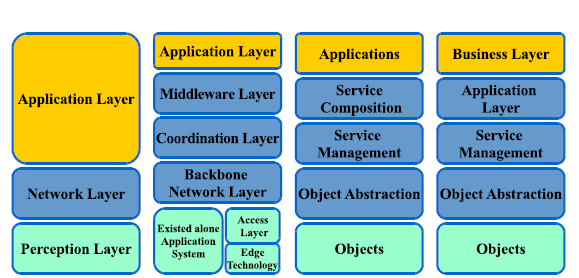
\includegraphics[width=0.75\textwidth]{Img/diagrama_capas.png}
    \caption{Arquitectura en capas característica de los ecosistemas IoT: capa de percepción (sensores), red (WLAN) y aplicación \cite{al2015internet}.}
    \label{fig:diagrama_capas}
\end{figure}

\subsection{Tecnologías de detección de presencia y sus limitaciones}
La correcta inferencia del contexto en un espacio inteligente está vinculada a la fiabilidad de la telemetría de presencia humana. Los sistemas tradicionales han dependido históricamente de transductores binarios de bajo coste, cuyas limitaciones físicas condicionan la estabilidad de las automatizaciones complejas.

\subsubsection{Sensores infrarrojos pasivos (PIR)}
Los dispositivos PIR operan mediante la captación de las variaciones de radiación térmica en el espectro infrarrojo dentro de su campo de visión. El elemento sensor, usualmente piroeléctrico, está segmentado en ranuras diferenciales cubiertas por una lente de Fresnel que enfoca la energía infrarroja. Cuando un cuerpo con una temperatura diferencial respecto al fondo cruza estas ranuras, el transductor genera una fluctuación de tensión que el circuito integrado interpreta como movimiento \cite{labeodan2015survey}.

Esta naturaleza física introduce dos limitaciones severas:
\begin{itemize}
    \item \textbf{Incapacidad de detección estática:} si el sujeto permanece inmóvil (por ejemplo, durante la lectura, el trabajo en escritorio o el sueño), la radiación térmica proyectada sobre el sensor piroeléctrico se vuelve constante, anulando la variación de tensión. Esto genera falsos negativos que interrumpen de forma anómala las automatizaciones.
    \item \textbf{Sensibilidad a gradientes térmicos:} al depender de la temperatura diferencial, los sensores PIR son vulnerables a falsos positivos provocados por corrientes de aire caliente, radiación solar directa sobre superficies interiores o el encendido automático de sistemas de climatización por convección.
\end{itemize}

\subsubsection{Sensores ultrasonidos}
Los sensores acústicos de presencia emiten ráfagas de ondas ultrasónicas de alta frecuencia (típicamente entre 30 kHz y 40 kHz) y miden el tiempo de vuelo (ToF) del eco reflejado o evalúan el desplazamiento de frecuencia provocado por el efecto Doppler al impactar sobre un objeto en movimiento. Aunque superan a los sensores PIR en la detección de movimientos axiales sutiles y no requieren línea de visión directa estricta, presentan una alta vulnerabilidad a interferencias acústicas ambientales, ruidos de conmutación y oscilaciones mecánicas de baja frecuencia generadas por electrodomésticos o tráfico exterior \cite{labeodan2015survey}.

\subsection{Fundamentos del radar de ondas milimétricas (mmWave)}
Para superar la naturaleza puramente binaria de los sensores convencionales, la inteligencia ambiental integrada en el perímetro residencial recurre a sistemas de radar de onda continua modulada en frecuencia (FMCW, por sus siglas en inglés) que operan en el espectro de las microondas de alta frecuencia, específicamente en la banda de 24 GHz \cite{soumya2023mmwave}. Aunque esta banda pertenece técnicamente al espectro de microondas (SHF), comercial e industrialmente suele catalogarse dentro de las tecnologías de ondas milimétricas (mmWave) por su principio de funcionamiento y el reducido tamaño de sus antenas integradas.

El principio de operación de un radar FMCW se basa en la emisión continua de una señal electromagnética cuya frecuencia varía linealmente en el tiempo siguiendo un patrón de rampa o \textit{chirp}. La señal reflejada por los obstáculos en el entorno es captada por la antena receptora del dispositivo. Debido al tiempo de propagación de la onda, existe un desfase temporal entre la señal emitida y la recibida en un instante dado, lo que genera una diferencia de frecuencia medible denominada frecuencia intermedia o de batido ($f_b$) \cite{rao2017introduction}.

El procesamiento analógico y digital de la señal intermedia en el propio microcontrolador del radar se ejecuta mediante la transformada rápida de Fourier (FFT). Este análisis espectral permite discretizar el espacio físico en celdas volumétricas o compuertas de distancia (\textit{range gates}), tal como se modela matemáticamente en la Ecuación \ref{eq:radar_range}:

\begin{equation}
\label{eq:radar_range}
R = \frac{c \cdot f_b \cdot T_c}{2 \cdot B}
\end{equation}

Donde $c$ representa la velocidad de la luz, $T_c$ es la duración del periodo de la rampa de frecuencia, y $B$ corresponde al ancho de banda de la modulación aplicada. 

\begin{figure}[H]
    \centering
    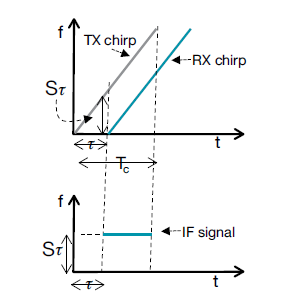
\includegraphics[width=0.45\textwidth]{Img/grafica_chirp.png}
    \caption{Representación en el dominio tiempo-frecuencia de las señales transmitidas (Tx) y recibidas (Rx) en un radar FMCW, ilustrando el retardo temporal $\tau$ y la frecuencia intermedia o de batido resultante \cite{rao2017introduction}.}
    \label{fig:grafica_chirp}
\end{figure}

Mediante la evaluación continua del desfase de fase de los ecos en compuertas de distancia milimétricas, los radares FMCW modernos, como el modelo HLK-LD2410, poseen la resolución necesaria para registrar variaciones submilimétricas en la superficie del cuerpo humano. Esta capacidad analítica faculta al sensor para detectar de manera ininterrumpida los movimientos torácicos asociados a la respiración y los micromovimientos vasculares periféricos, manteniendo el estado de presencia activo incluso si el usuario se encuentra en reposo absoluto o durmiendo, eliminando de raíz los falsos negativos inherentes a la sensórica piroeléctrica \cite{turppa2020vital} (véase la Figura \ref{fig:pir_vs_mmwave}).

\begin{figure}[H]
    \centering
    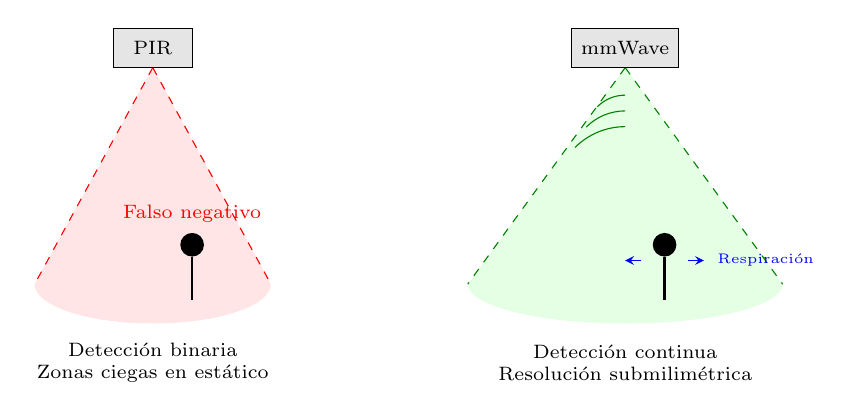
\begin{tikzpicture}
    
    % PIR Sensor
    \begin{scope}[shift={(0,0)}]
        % Draw cone first (background)
        \fill[red!20, opacity=0.5] (0,2.75) -- (-1.5,0) arc(180:360:1.5 and 0.5) -- cycle;
        \draw[red, dashed] (0,2.75) -- (-1.5,0);
        \draw[red, dashed] (0,2.75) -- (1.5,0);
        
        % Draw sensor box on top
        \node[draw, rectangle, fill=gray!20, minimum width=1cm, minimum height=0.5cm, font=\scriptsize] (pir) at (0,3) {PIR};
        
        \node[font=\scriptsize, align=center] at (0,-1) {Detección binaria\\Zonas ciegas en estático};
        
        % Person
        \fill[black] (0.5,0.5) circle (0.15); % head
        \draw[thick] (0.5,0.35) -- (0.5,-0.2); % body
        \node[font=\scriptsize, red] at (0.5, 0.9) {Falso negativo};
    \end{scope}
    
    % mmWave Sensor
    \begin{scope}[shift={(6,0)}]
        % Draw cone first (background)
        \fill[green!20, opacity=0.5] (0,2.75) -- (-2,0) arc(180:360:2 and 0.5) -- cycle;
        \draw[green!50!black, dashed] (0,2.75) -- (-2,0);
        \draw[green!50!black, dashed] (0,2.75) -- (2,0);
        
        % Draw sensor box on top
        \node[draw, rectangle, fill=gray!20, minimum width=1cm, minimum height=0.5cm, font=\scriptsize] (mmw) at (0,3) {mmWave};
        
        % Waves
        \draw[green!50!black] (0,2.4) arc(90:135:0.5);
        \draw[green!50!black] (0,2.2) arc(90:135:0.7);
        \draw[green!50!black] (0,2.0) arc(90:135:0.9);
        
        \node[font=\scriptsize, align=center] at (0,-1) {Detección continua\\Resolución submilimétrica};
        
        % Person
        \fill[black] (0.5,0.5) circle (0.15); % head
        \draw[thick] (0.5,0.35) -- (0.5,-0.2); % body
        
        % Breathing arrows
        \draw[blue, -stealth] (0.2, 0.3) -- (0.0,0.3);
        \draw[blue, -stealth] (0.8, 0.3) -- (1.0,0.3);
        \node[font=\tiny, blue, anchor=west] at (1.05, 0.3) {Respiración};
    \end{scope}
    
    \end{tikzpicture}
    \caption{Representación conceptual de las limitaciones volumétricas de los sensores PIR tradicionales frente a la detección continua de micromovimientos de los radares mmWave.}
    \label{fig:pir_vs_mmwave}
\end{figure}

\subsection{Protocolos de comunicación IoT}
La integración de nodos distribuidos heterogéneos dentro de una infraestructura local requiere el análisis de los protocolos de transporte y las capas de enlace físico para garantizar la baja latencia y la inmunidad al ruido electromagnético residencial.

\subsubsection{Comparativa de tecnologías inalámbricas}
Las tecnologías de red aplicadas al ámbito del IoT se segmentan principalmente por su alcance, ancho de banda y consumo energético. Las redes WAN de baja potencia (LPWAN), como LoRaWAN, destacan por su gran alcance kilométrico y alta penetración en estructuras densas, propiedades críticas en sistemas de monitorización industrial distribuidos o control de aparcamientos urbanos \cite{mekki2019comparative}. No obstante, sus severas restricciones en la tasa de transferencia de datos y los ciclos de trabajo limitados (\textit{duty cycle}) invalidan su uso para telemetría domótica en tiempo real, donde se requiere el envío constante de flujos analógicos por segundo.

Para entornos domésticos confinados, los protocolos de red en malla basados en el estándar IEEE 802.15.4, como Zigbee, ofrecen un balance óptimo entre consumo y direccionamiento de nodos. Sin embargo, su integración requiere el despliegue de pasarelas específicas de traducción de protocolos. Por este motivo, para el diseño de nodos de instrumentación continua con alimentación permanente, el uso del estándar IEEE 802.11b/g/n (Wi-Fi) sobre la banda de 2.4 GHz resulta el más eficiente. Proporciona una infraestructura de red local preexistente con un ancho de banda elevado que asimila las ráfagas de datos analógicos de los microcontroladores sin introducir cuellos de botella lógicos.

\begin{figure}[H]
    \centering
    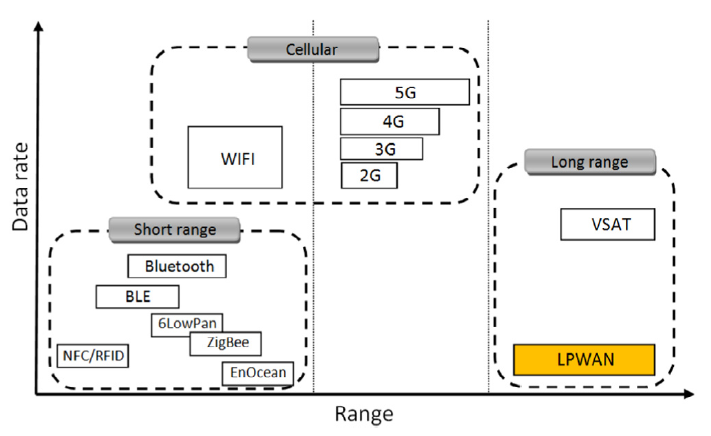
\includegraphics[width=0.7\textwidth]{Img/grafica_protocolos.png}
    \caption{Comparativa de tecnologías inalámbricas para ecosistemas IoT en función de su tasa de transferencia de datos frente a su alcance efectivo \cite{mekki2019comparative}.}
    \label{fig:grafica_protocolos}
\end{figure}

\subsubsection{El protocolo de transporte MQTT}
Sobre la capa de transporte TCP/IP de la red Wi-Fi, el protocolo de mensajería MQ Telemetry Transport (MQTT) se establece como el estándar de facto para arquitecturas perimetrales eficientes. MQTT opera bajo un modelo de publicación/suscripción desacoplado mediado por un agente central o \textit{broker} \cite{al2015internet}, tal y como se esquematiza en la Figura \ref{fig:mqtt_pubsub}.

\begin{figure}[H]
    \centering
    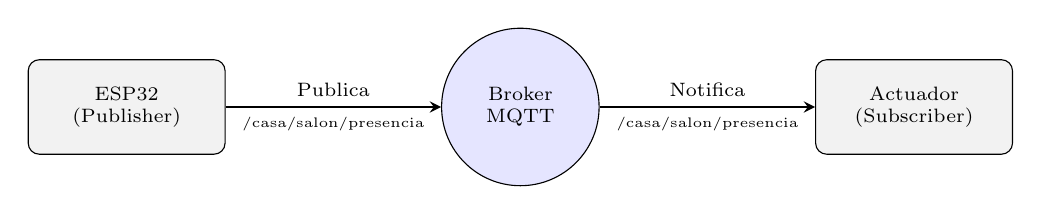
\begin{tikzpicture}[
        broker/.style={draw, circle, minimum size=2cm, align=center, fill=blue!10, font=\scriptsize},
        nodebox/.style={draw, rectangle, rounded corners, minimum width=2.5cm, minimum height=1.2cm, align=center, fill=gray!10, font=\scriptsize},
        arrow/.style={thick, -stealth}
    ]
    
    \node[nodebox] (pub) at (0,0) {ESP32\\(Publisher)};
    \node[broker] (broker) at (5,0) {Broker\\MQTT};
    \node[nodebox] (sub) at (10,0) {Actuador\\(Subscriber)};
    
    \draw[arrow] (pub) -- node[anchor=south, font=\scriptsize] {Publica} node[anchor=north, font=\tiny] {/casa/salon/presencia} (broker);
    \draw[arrow] (broker) -- node[anchor=south, font=\scriptsize] {Notifica} node[anchor=north, font=\tiny] {/casa/salon/presencia} (sub);
    
    \end{tikzpicture}
    \caption{Arquitectura de publicación y suscripción del protocolo MQTT.}
    \label{fig:mqtt_pubsub}
\end{figure}

Frente a protocolos síncronos pesados (como HTTP\slash REST), MQTT ofrece ventajas esenciales para el proyecto:
\begin{itemize}
    \item \textbf{Reducido sobrecoste de protocolo (\textit{overhead}):} la cabecera fija del protocolo es de únicamente 2 bytes, reduciendo el consumo de ancho de banda y los tiempos de serialización en procesadores limitados como el ESP32.
    \item \textbf{Gestión de la calidad de servicio (QoS):} permite parametrizar el nivel de entrega de los mensajes (QoS 0, QoS 1 o QoS 2), asegurando la llegada de eventos críticos relativos a la seguridad perimetral frente a telemetrías ambientales repetitivas.
    \item \textbf{Mecanismo de testamento (\textit{Last Will and Testament}):} permite al \textit{broker} notificar de forma proactiva y automática la desconexión abrupta de un nodo sensor por fallo eléctrico o pérdida de Wi-Fi, habilitando la ejecución inmediata de rutinas de contingencia en el servidor central local.
\end{itemize}

\subsection{Soluciones comerciales y antecedentes}
El mercado actual de consumo ofrece una amplia gama de ecosistemas domóticos propietarios desarrollados por corporaciones tecnológicas internacionales. Plataformas basadas en los ecosistemas de Tuya/Smart Life, Google Home o Philips Hue proporcionan interfaces de usuario pulidas y compatibilidad simplificada mediante el modelo \textit{Plug-and-Play}. Sin embargo, un análisis de ingeniería revela deficiencias estructurales en estas soluciones:

\begin{itemize}
    \item \textbf{Aislamiento en silos tecnológicos:} los fabricantes tienden a restringir la interoperabilidad nativa, forzando al usuario a depender de pasarelas de traducción propietarias y aplicaciones de software independientes que complican la unificación de datos.
    \item \textbf{Dependencia de la nube:} la lógica de conmutación y la ejecución de las automatizaciones de estas soluciones comerciales se procesan en servidores remotos. Si la conexión a internet del hogar se degrada o el servidor del proveedor experimenta una interrupción del servicio, el entorno pierde por completo sus capacidades autónomas.
    \item \textbf{Monetización e intrusión en la privacidad:} el almacenamiento masivo de históricos de presencia, hábitos horarios y perfiles acústicos en infraestructuras externas plantea serios dilemas éticos y legales bajo normativas de protección de datos, al delegar la custodia de información sensible a terceros cuyos modelos de negocio suelen incluir la explotación analítica de datos agregados \cite{perera2014context}.
\end{itemize}

Frente a estos antecedentes comerciales, las arquitecturas de código abierto de integración local como Home Assistant y ESPHome plantean una alternativa sólida. Permiten la unificación de hardware heterogéneo bajo una capa de abstracción común operada de forma local, devolviendo el control operativo y la privacidad absoluta de los datos al perímetro de la vivienda.

Establecido el estado del arte y justificadas las ventajas del procesamiento local y la sensórica avanzada, el siguiente capítulo abordará la definición formal del problema, detallando los requisitos funcionales y no funcionales que guiarán el diseño y desarrollo de la solución propuesta.